
Outro algoritmo frequentemente referenciado na literatura é o C99 o qual é baseado em uma matriz de \textit{ranking} das similaridades. Embora muitos trabalhos utilizem a coesão léxica do texto, para pequenos segmentos pode não ser não é confiável, pois a ocorrência adicional de uma palavra pode causar certo impacto e alterar o cálculo da similaridade~\cite{Choi2000}. Além disso, o estilo da escrita normalmente não é constante em todo o texto. Por exemplo, textos iniciais dedicados a introdução costumam apresentar menor coesão do que trechos dedicados a um tópico específico. Portanto, comparar a similaridade entre trechos de diferentes regiões não é apropriado. Devido a isso, as similaridades não podem ser comparadas em valores absolutos. Então, contorna-se esse problema fazendo uso de matrizes de similaridade para encontrar os segmentos de texto. Para isso, o C99 constrói uma matriz que contém as similaridades de todas as unidades de informação (normalmente sentenças ou parágrafos). 

%%%%%% 
%%%%%% 

Na Figura~\ref{fig:matrix-similarity} é mostrado um exemplo de uma matriz de similaridade onde a intensidade do ponto($i,j$) representa a similaridade entre as sentenças $i$ e $j$. Observa-se que a matriz é simétrica, assim cada ponto na linha diagonal representa a similaridade quanto $i = j$ (ou seja, com a mesma sentença) e revela quadrados com maior concentração de pontos ao longo da diagonal. Essas regiões indicam porções de texto com maior coesão léxica.


  %--- Figura Visão Geral ---
  \begin{figure}[!h]
	  \centering
	  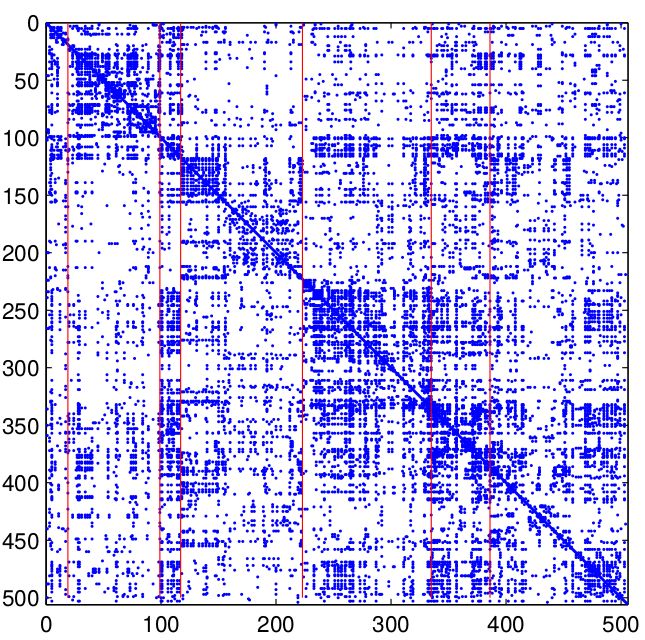
\includegraphics[width=1\textwidth]{conteudo/capitulos/figs/c99-ranking-matrix.png}
	  \caption{\textit{DotPlot} da similaridade entre sentenças onde as linha verticais representam segmentos reais.}
	  \label{fig:matrix-similarity}
  \end{figure}



%%%%%%%%%%%%%%%%%%%%%%%
% - Falar do esquema de ranking;
% - Imagem com os passos e máscara 3x3;
%%%%%%%%%%%%%%%%%%%%%%%

Em seguida, cada valor na matriz de similaridade é substituído por seu \textit{ranking local}. Para cada elemento da matriz, seu \textit{ranking} é o número de elementos vizinhos com valor de similaridade menor que o seu. Então, cada elemento e comparado com seus vizinhos dentro de uma região denominada máscara.
% 
% 
Na Figura~\ref{fig:a} é destacado um quadro 3~x~3 de uma matriz em que cada elemento é a similaridade entre duas unidades de informação. Tomando como exemplo o elemento com valor $0,5$, a mesma posição na matriz de \textit{rankings} terá o valor $4$, pois esse é o número de vizinhos com valores inferiores a $0,5$ dentro do quadro analisado na matriz de similaridades. Da mesma forma, na Figura~\ref{fig:b} para o valor $0,2$ a matriz de \textit{rankings} conterá o valor $1$ na mesma posição. Após a construção da matriz de ranking obtêm-se um maior contraste entre facilitando a detecção de limites quando a queda de similaridade entre sentenças é mais sutil.

\begin{figure}[!h]
	\centering     %%% not \center

	\subfigure[Passo 1]{\label{fig:a}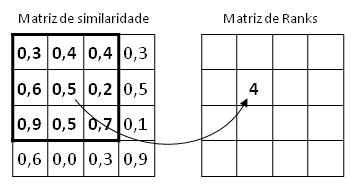
\includegraphics[width=60mm]{conteudo/capitulos/figs/exemplo-matrix-rank-A.png}}
	\subfigure[Passo 2]{\label{fig:b}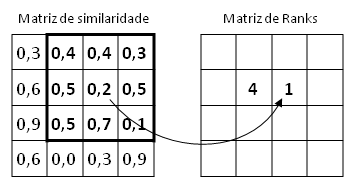
\includegraphics[width=60mm]{conteudo/capitulos/figs/exemplo-matrix-rank-B.png}}
	
	\caption{Exemplo de construção de uma matriz de rankings.%~\cite{Choi2000}.
	}
	\label{fig:exemplomatrixrank}
\end{figure}
% -< Colocar uma explicação mais detalhada para esses passos




Finalmente, com base na matriz de \textit{ranking}, o C99 utiliza um método de \textit{clustering} baseado no algoritmo de \textit{DotPloting} que usa regiões com maior densidade em uma matriz de similaridades para determinar como os segmentos estão distribuídos. Um segmento é definido por duas sentenças $i$ e $j$ que representam uma região quadrada ao longo da diagonal da matriz. Calcula-se a densidade dessa região como mostrado na Equação~\ref{equ:densidade-c99}. Seja $s_{i,j}$ a somatória dos \textit{rakings} de um segmento e $a_{i,j}$ sua área interior. Seja $B = \{b1,...,b_m\}$ a lista de $m$ segmentos e$s_k$  $a_k$ são a somatória dos valores dos rankings e a área de um segmento $k$ em $B$. Então, a densidade é computada por: 

\begin{equation}
D = \frac{\sum_{k=1}^m s_k}{\sum_{k=1}^m a_k}
\label{equ:densidade-c99}
\end{equation}


O processo incia com um único segmento formado por todas as sentenças do documento e o divide recursivamente em $m$ segmentos. Cada passo divide um dos segmentos em B no ponto $ij$ que maximiza D~(Equação \ref{equ:densidade-c99}). O processo ser repte até atingir o número de segmento desejados ou um limiar de similaridade.
 







*******************************************





Mede-se a profundidade de um vale por

A identificação de um limite se da pela atribuição de uma medida de profundidade há cada final de sentença. Para um ponto i 









... que indica uma diminuição da similaridade entre os blocos adjacentes. 







% A partir desses conceitos, vários algoritmos foram propostos baseados na ideia de que um segmento pode ser identificado pela análise das palavras que o compõe~\cite{Chen2017,Ferret2009,Sakahara2014}.
% Acho que dá pra melhorar essas referências;


% vários algoritmos foram propostos baseados na ideia de que um segmento pode ser identificado pela análise das palavras que o compõe~\cite{Chen2017,Ferret2009,Sakahara2014}.


% A partir desses conceitos, um dos primeiros algoritmos baseados na ideia que um segmento pode ser identificado pela análise das palavras que o compõe foi o \textit{TextTiling}. O \textit{TextTiling} é um algoritmo baseado em janelas deslizantes, em  que, para cada candidato a limite, analisa-se o texto circundante. Um limite ou quebra entre segmentos é identificado sempre que a similaridade entre as unidades que antecedem e precedem o ponto candidato cai abaixo de um limiar. O \textit{TextTiling} recebe uma lista de candidatos a limite, usualmente finais de parágrafo ou finais de sentenças. Para cada posição candidata são construídos 2 blocos, um contendo sentenças que a precedem e outro com as que a sucedem. O tamanho desses blocos é um parâmetro a ser fornecido ao algoritmo e determina o tamanho mínimo de um segmento. Em seguida, os blocos de texto são representados por vetores que contém as frequências de suas palavras. Então, usa-se cosseno (Equação~\ref{equ:cosine}) para calcular a similaridade entre os blocos adjacentes a cada candidato e identifica-se uma transição entre segmentos pelos vales na curva de dissimilaridade.



% Então, usa-se cosseno (Equação~\ref{equ:cosine}) para calcular a similaridade entre os blocos adjacentes a cada candidato e identifica-se uma transição entre segmentos pelos vales na curva de dissimilaridade.




% -- Porque cosseno
% Uma vez que a coesão léxica é pressuposto básico da maioria dos algoritmos, o cálculo da similaridade entre unidades de informação é fundamental. Uma medida de similidade frequentemente utilizada é o cosseno, apresentada na Equação~\ref{equ:cosine}, onde dadas duas unidades de informação, $x$ e $y$, $f_{x,j}$ é a frequência do termo $j$ em $x$ e $f_{y,j}$ é a frequência do termo $j$ em $y$.

% \begin{equation}
	% Sim(x,y) = \frac
	% {\Sigma_j f_{x,j} \times f_{y,j}}
	% {\sqrt{\Sigma_j f^2_{x,j} \times \Sigma f^2_{y,j}}}
	% \label{equ:cosine}
% \end{equation}



% --> falar um pouco sobre TT e C99, sobre como foram pioneiros, influenciáram muitos outros e são empregrados até hoje;




Entre os principais trabalhos da literatura, podemos citar o \textit{TextTiling} que foi um dois primeiros trabalhos em segmentação textual proposto por Fulano em 19XX. Tem como princípio a similaridade com







Entre os trabalhos tradicionais da literatura podemos citar o  \textit{TextTiling}~\cite{Hearst1994} e o \textit{C99}~\cite{Choi2000}. 

O \textit{TextTiling} é um algoritmo baseado em janelas deslizantes, em  que, para cada candidato a limite, analisa-se o texto circundante.



TT foi pioneiro sendo um dos primeiros a implementar um algoritmo baseado em coesão lexica proposto por Kosima, mas só que melhor pq ... (ver no artigo do próprio Hearst)
Kosima usa uma rede e o TT usa repetição de palavras (cosine)

baseou-se no trabalho de Kosima que usa uma rede semântica para calcular a coesão léxica de uma janela de palavras  


TT influenciou o Segmenter (Kan et al., 1998)??
TT influenciou o Galley et al.’s (2003)!!



Um texto é uma 
o significado de um palavra somente pode ser determinado quando está dentro de um contexto.




% Um dos primeiros algoritmos a aplicar essa técnica foi proposto por Kosima. Em seu trabalho, utilizou uma rede semântica para calcular a coesão léxica de uma janela de palavras. Contudo, sua adaptação para outros domínios dependia da construção de uma rede adequada. 


% ==========  Janelas deslizantes  ==========

% Kosima uniu as tecnicas de SW e CL.
% Os algoritmos que se baseiam no cálculo da similaridade entre sentenças, frequentemente o fazem por meio de janelas deslizantes, onde se verifica a frequência dos termos em um fragmento do documento. Inicialmente, estabelece-se a partir do início do texto, um \textit{range} de $w$ termos, chamado janela que é deslocada $k$ termos adiante até o final do texto. A cada passo, calcula-se a coesão léxica das palavras contidas na janela. Kosima demonstrou que há uma estreita correlação entre quedas na coesão léxica em janelas de texto e a transição de assuntos. Em seu trabalho, calculou a coesão léxica de uma janela de palavras usando \textit{spreading activation} em uma rede semântica especialmente elaborada para o idioma Inglês. Contudo, sua implementação de um algoritmo para outros domínios dependia da construção de uma rede adequada. 



% Os algoritmos que se baseiam no cálculo da similaridade entre sentenças, frequentemente o fazem por meio de janelas deslizantes, onde se verifica a frequência dos termos em um fragmento do texto. Inicialmente, estabelece-se um range de $w$ termos, chamado janela, e calcula-se a coerência léxica das palavras contidas nessa janela. Em seguida, esta é deslocada $k$ termos adiante e novamente se calcula a coerência léxica de seus termos. Repete-se esse processo até o final do texto. 


% Os algoritmos que se baseiam no cálculo da similaridade entre sentenças, frequentemente o fazem por meio de janelas deslizantes, onde se verifica a frequência dos termos em um fragmento do texto. Inicialmente, estabelece-se um range de $w$ termos, chamado janela, e calcula-se a coerência léxica das palavras contidas nessa janela. Em seguida, esta é deslocada $k$ termos adiante até o final do texto e calcula-se ao coerência léxica de cada janela. Quando a co



% e calcula-se a coerência léxica das palavras contidas nessa janela. Em seguida, esta é deslocada $k$ termos adiante até o final do texto e calcula-se ao coerência léxica de cada janela. Quando a co




Trocar o "Uma vez que a coesão léxica é pressuposto básico" por "outra forma de de calcula a similaridade entre sentenças e "

ou no final justificar que é melhor que a do cozima por ser independente de domínio.














***************************
# Bayesian Unsupervised Topic Segmentation
***************************

- Descreve uma abordagem Bayesiana à segmentação textual;
- 
- Impossibilidade de combinar cue-frases com as métricas tradicionais (cosine)
- {enquadra a coesão léxica em um contexto Bayesiano}
- usa programação dinâmica

"The Bayesian framework provides a principled way to incorporate additional features such as cue phrases, a powerful indicator of discourse structure"

%  ----------------------------------------

"We formalize lexical cohesion in a generative model in which the text for each segment is produced by a distinct lexical distribution." 

%  ----------------------------------------

"More formally, we treat the words in each sentence as draws from a language model associated with the topic segment. This is related to topic-modeling methods such as latent Dirichlet allocation (LDA; Blei et al. 2003), but here the induced topics are tied to a linear discourse structure. This property enables a dynamic programming solution to find the exact maximum-likelihood segmentation." 

%  ----------------------------------------


"Lexical cohesion can be placed in a probabilistic context by modeling the words in each topic segment as draws from a multinomial language model associated with the segment."

"Formally, if sentence t is in segment j, then the bag of words xt is drawn from the multinomial language model θ j."

%  ---------------------------------------- 

This is similar in spirit to hidden topic models such as latent Dirichlet allocation (Blei et al., 2003), but rather than assigning a hidden topic to each word, we constrain the topics to yield a linear segmentation of the document.

%  ---------------------------------------- 

"We model cue phrases as generated from a separate multinomial that is shared across all topics and documents in the dataset"
As frases-pista vem de um único modelo generativo.

%  ---------------------------------------- 

"This is achieved by biasing the selection of samples towards boundaries with known cue phrases"
{Isto é conseguido através da influência da seleção de amostras em direção a fronteiras com frases conhecidas}

%  ---------------------------------------- 

{As palavras que formam a sentença t em um segmento j provem de um modelo de linguagem multinomial θ j}

%  ---------------------------------------- 


"They then build a linear segmentation by adding a switching variable to indicate whether the topic distribution for each sentence is identical to that of its predecessor. Unlike Purver et al., we do not assume a dataset in which topics are shared across multiple documents; indeed, our model can be applied to single documents individually."

{Detecta-se um limite entre sentenças, quando a distribuição de tópicos entre elas for diferente}

%  ---------------------------------------- 


para as frases pistas, o modelo é adaptado para refletir essa ideia. Muda-se a probabilidade de ser um limite quando for uma pista.

fulano mostra que a coesão léxica pode ser enquadrada em um contexto bayesiano modelando as palavras em cada tópico como 







% Galley et al. (2003) encontra as pistas minerando segmentos rotulados em busca de palavras que ocorrem próximas aos limites; Elsner and Charniak (2008) construíram uma lista de frases-pista manualmente;

Fulano e fulana apresentam um método para aproveitar essas pistas

% -< Alguns termos são usados para expressar uma estrutura do texto
% -< Alguns termos são usados para expressar uma estrutura do texto

% -< Alguns termos são usados em tópicos específicos, mas outros são neutros em relação aos tópicos sendo usados para expressar uma estrutura do discurso.

% Beltrano mostra que essas palavras não pertencem a um tópico específico, mas são neutras em relação a algum assunto sendo usadas para expressar a estrutura do discurso.


Fulano e fulana mostram em seu trabalho que a coesão léxica pode ser enquadrada em um contexto bayesiano onde as palavras de um segmento surgem de um modelo de linguagem multinomial o qual é associado a um tópico.
% -< e com isso aproveitam as pistas.


onde as palavras de um segmento surgem de um modelo de linguagem multinomial o qual é associado a um tópico.

onde as palavras de um segmento surgem de modelo generativo em que o texto de cada segmento é produzido por uma distribuição léxica distinta. 











% O método BayesSeg~\cite{} aborda a coesão léxica em um contexto bayesiano onde as palavras de um segmento surgem de um modelo generativo em que o texto de cada segmento é produzido por uma distribuição léxica distinta. Assim, considera-se que as palavras de cada sentença surgem de um modelo de linguagem multinomial o qual está associado ao assunto.		








fulano e fulana apresentam uma abordagem baseada em um modelo bayesiano que permite aproveitar esses indicadores para encontrar segmentos melhores.







1 - TextSeg
2 - MinCut
3 - BayesSeg


Lexical cohesion e.g., 
	- Utiyama and Isahara,     2001; {TextSeg}
	- Galley et al.            2003; {LCSeg}
	- Malioutov and Barzilay,  2006  {}




% Utiyama ==>
% https://github.com/jacobeisenstein/bayes-seg/tree/master/baselines/textseg-1.211

